\section{Stationary distributions}\label{section: stationary distributions}
We now consider the hunger game process for nonabsorbing Markov chains, 
so that chips are never inserted or removed.

Say that a vector $\v$ is stationary under $P$ if $\v P = \v$,
or equivalently $\v H = \v(P-I) = {\bf 0}$.
Let $E$ be the space of vectors that are stationary under $P$,
or equivalently the nullspace of $H$.
When the Markov chain is irreducible,
so that there is a unique stationary distribution $\ppi$,
$E$ is the 1-dimensional subspace of $\R^n$
consisting of multiples of $[\ppi(1),\dots,\ppi(n)]$.

Define the \textbf{firing vector} $\v$ 
after $N$ steps of a hunger game process 
to be the vector whose $i$th component $\v_i$ is 
the number of times $H_i$ was added to $\h$, 
i.e.\ the number of times the chip fired to vertex $v_i$.
The following theorem demonstrates that 
the normalized firing vector $\frac{\v}{N}$ 
approximates the unique stationary distribution $\ppi$ 
of an irreducible finite Markov chain 
within a distance proportional to $N^{-1}$.

\begin{theorem}\label{theorem: irreducible fidelity converge stationary}
Given a hunger game process on an irreducible finite Markov chain, 
let $\v^{(N)}$ be the firing vector after $N$ steps.
Then the sequence of normalized firing vectors 
$\left\{\frac{1}{N}\v^{(N)}\right\}$ converges to 
the unique stationary distribution $\ppi$, 
where there exists a constant $C$ such that for all $N$, 
the normalized firing vector is within distance $\frac{C}{N}$ of $\ppi$ 
in the $L^1$ metric.
\end{theorem}
\begin{proof}
Since the Markov chain is irreducible, 0 is a simple eigenvalue of $H$.
Let $c$ be the maximum of $1/|\lambda|$
where $\lambda$ ranges over the nonzero eigenvalues of $H$.
For $d \in \R$, let $U_d = \{\x \mid \x_1 + \cdots + \x_n = d\}$, 
where there are $n$ states in the Markov chain.
The fact that 0 is a simple eigenvalue of $H$
and that every other eigenvalue has norm at least $1/c$
implies that the restriction of $H$
to an affine map from $U_1$ to $U_0$ is invertible,
and that if two points $\p^{(1)}, \p^{(2)}\in U_0$ 
are within distance $\varepsilon$, then 
their two preimages $\x^{(1)},\x^{(2)}\in U_1$
are within distance $c\varepsilon$ of each other.

It follows that if we have a point $\p\in U_0$ 
within distance $\varepsilon$ of $\mathbf{0}$, 
the preimages $\v,\ppi\in U_1$ of $\p$ and $\mathbf{0}$, respectively, 
are within distance $c\varepsilon$ of each other.
As a result, $\v$ is within distance $c\varepsilon$ 
of the stationary distribution $\ppi$.

By \cref{lemma: hunger bounded}\,,
during any hunger game process hunger remains bounded, 
so the change in hunger after $N$ steps, given by $\v^{(N)} H$, 
is within a bounded distance, say $b$, of $\mathbf{0}$.
This implies $\left(\frac{1}{N}\v^{(N)}\right)H$ is 
within distance $\frac{b}{N}$ of $\mathbf{0}$, 
which implies the normalized firing vector $\frac{1}{N}\v^{(N)}$ 
is within distance $\frac{bc}{N}$ of a stationary distribution $\ppi$.
Setting $C=bc$ yields our desired result.
\end{proof}
\begin{remark}\label{remark: fidelity converge stationary single absorbing}
As the only time irreducibility was assumed 
in \cref{theorem: irreducible fidelity converge stationary} was 
when we claimed the Markov chain had a unique stationary distribution $\ppi$,
the result holds for any finite Markov chain with a unique stationary distribution.
Namely, it also works for absorbing Markov chains 
with a single absorbing state $v_k$, where $\ppi$ is the vector 
with a 1 corresponding to state $v_k$ and 0s elsewhere.
\end{remark}

When a unique stationary distribution exists, 
the stationary distribution represents, in the long run, 
the probability distribution of the chain being at each particular state, 
or the occupation frequency distribution.
As a result, \cref{theorem: irreducible fidelity converge stationary} 
illustrates that the normalized firing vector, 
which counts how many times the chip arrives at each state in the hunger game, 
approximates the occupation frequency distribution 
within a discrepancy proportional to $N^{-1}$, 
better than the $N^{-1/2}$ discrepancy expected 
from repeated samplings of the corresponding random process.

\begin{example}\label{example: stationary distribution}
The Markov chain described in \cref{example: 3 hunger} is irreducible, 
and has unique stationary distribution 
$\ppi=\left[\frac{1}{3},\frac{1}{3},\frac{1}{3}\right]$, 
as shown in \cref{fig:ex stationary}\,.
\begin{figure}[htbp]
    \centering
    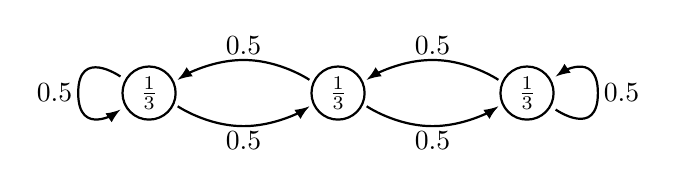
\begin{tikzpicture}[scale=0.6,font=\normalsize,baseline,thick]
        \foreach \x in {1,...,3} {
            \filldraw[color=black,fill=white,thick] (4*\x,0) circle (16pt);
            \node at (4*\x,0) {$\frac{1}{3}$};
        }
        % Left arrows
        \foreach \x in {2,3} {
            \draw [->,>=latex] plot [smooth,tension=1] coordinates {(4*\x-0.866*0.7,0.4*0.7) (4*\x-2,0.7) (4*\x-4+0.866*0.7,0.4*0.7)};
        }
        % Right arrows
        \foreach \x in {1,2} {
            \draw [->,>=latex] plot [smooth,tension=1] coordinates {(4*\x+0.866*0.7,-0.4*0.7) (4*\x+2,-0.7) (4*\x+4-0.866*0.7,-0.4*0.7)};
        }
        \node at (6,1) {0.5};
        \node at (10,1) {0.5};
        \node at (6,-1) {0.5};
        \node at (10,-1) {0.5};
        \draw [->,>=latex] plot [smooth,tension=5] coordinates {(4-0.866*0.7,0.5*0.7) (4-1.5,0) (4-0.866*0.7,-0.5*0.7)};
        \node at (2,0) {0.5};
        \draw [->,>=latex] plot [smooth,tension=5] coordinates {(12+0.866*0.7,-0.5*0.7) (12+1.5,0) (12+0.866*0.7,0.5*0.7)};
        \node at (14,0) {0.5};
    \end{tikzpicture}
    \caption{The unique stationary distribution $\ppi$ of a doubly-reflecting random walk}
    \label{fig:ex stationary}
\end{figure}
From \cref{example: 3 hunger} we know that 
the states are visited periodically in the order 1, 2, and 3, 
so the firing vector starting at $\mathbf{h}=\mathbf{0}$ is given by
\begin{align*}
    \mathbf{v}^{(N)} = \left[\left\lfloor\dfrac{N+2}{3}\right\rfloor,\left\lfloor\dfrac{N+1}{3}\right\rfloor,\bigg\lfloor\dfrac{N}{3}\bigg\rfloor\right],
\end{align*}
or equivalently
\begin{align*}
    \mathbf{v}^{(3M)} &= \left[M,M,M\right] \\
    \mathbf{v}^{(3M+1)} &= \left[M+1,M,M\right] \\
    \mathbf{v}^{(3M+2)} &= \left[M+1,M+1,M\right].
\end{align*}
\cref{theorem: irreducible fidelity converge stationary} guarantees 
the existence of some constant $C$ such that 
the normalized firing vector $\frac{1}{N}\mathbf{v}^{(N)}$ 
is within $\frac{C}{N}$ of $\ppi$ for all $N$.
In fact, we will show $C=\frac{4}{3}$ is the minimal such constant.
Then for $N=3M$, the normalized firing vector is 
$\left[\frac{1}{3},\frac{1}{3},\frac{1}{3}\right]$, so there is no discrepancy,
while for $N=3M+1$ the normalized firing vector is 
$\left[\frac{M+1}{3M+1},\frac{M}{3M+1},\frac{M}{3M+1}\right]$, 
whose discrepancy from $\ppi=\left[\frac{1}{3},\frac{1}{3},\frac{1}{3}\right]$ 
is $\frac{4/3}{3M+1}=\frac{C}{N}$.
Similarly for $N=3M+2$.

In general, however, unlike in this example, 
the sequence of states visited need not be periodic, 
as the transition probabilities can be irrational.
\end{example}
